% -*- TeX-master: "main.tex" -*-

% Resultate, Bewerung und Ausblick
\chapter{Results}
\label{ch:results}

% Zielerreichung
\section{Achievement of Objectives}

In this chapter, the objectives set in section \ref{goals} will be reviewed.

\subsection{Merging contributions}
\label{sec:merging}
At the beginning of this project, various third-party contributions were pending
a code review, due to being ignored during the exam session preceding this
semester.

Since those contributions would conflict with the refactorings needed before
work on the extension API started, a block of time was reserved for code
reviews at the beginning of this project (see figure \ref{img:schedule} on page
\pageref{img:schedule}).

To avoid receiving more contributions while refactoring the code, the
following notice was added to qutebrowser's contribution guidelines:

\begin{quote}
Important: \emph{Currently, bigger changes are going on in qutebrowser, as
part of a student research project about adding a plugin API to qutebrowser
and moving a lot of code from the code into plugins.} Due to that, bandwidth
for pull request review is currently very limited, and contributions might lead
to merge conflicts due to ongoing refactorings.
\end{quote}

The impact of such a notice is hard to measure, but pull requests (where
contributors request their changes to be pulled into the main repository)
continued to be opened regularly throughout the project.

Thus, the decision was taken to continue with the next step despite many
remaining open contributions, and only merge new contributions if they are
trivial enough.

\subsection{Refactorings}
In section \ref{sec:goals-refactorings}, three major refactorings related to the
extension API were identified:

\begin{itemize}
  \item qutebrowser should introduce ``gradual typing'' and a type checker such
    as mypy into its toolchain. This goal was fully achieved despite some issues
    with third-party projects (which were fixed as part of this project), see
    section \ref{sec:mypy}.
  \item The documentation toolchain used in qutebrowser should be switched to
    the Sphinx tool. Some work on this was started by an external contributor,
    but not finished in time, which was identified as one of the possible risks
    in section \ref{sec:risks}. To remedy this, Sphinx was introduced alongside
    the existing documentation toolchain, and only used to document the
    extension API (see appendix \ref{ch:sphinx}). The author of this report
    (Florian~Bruhin) will meet with the external contributor (Fritz~Reichwald)
    at the \nth{35} Chaos Communication
    Congress\footnote{\url{https://en.wikipedia.org/wiki/Chaos_Communication_Congress}}
    after this project is done (December 27th to 30th, 2018).
    There, they plan to finish migrating the entire existing documentation to
    the Sphinx tool.
  \item The ``object registry'' (\texttt{objreg} module) in qutebrowser should
    be refactored, as it has various issues and influences the public API. Work
    on this goal was started but not completed due to some deeper issues with
    its implementation\footnote{See \url{https://github.com/qutebrowser/qutebrowser/issues/640\#issuecomment-443143463}}.
    Fixing these issues properly would take more time than anticipated, thus this
    refactoring was not completed. However, care was taken to not add the object
    registry to the API exposed to extensions, so this change can still be done
    after the API has been implemented.
\end{itemize}

The initial refactoring goals were only met partially -- however, it was
possible to continue with implementing the extension API despite that. Care was
taken to make sure that work absolutely necessary for the extension API was
finished.

\subsection{Extension API}

While the extension API resulting from this work is rather minimal, it is
already quite powerful: As described in section \ref{sec:components}, it allowed
various components to be moved from qutebrowser's core to use the extension API.
It also implements dynamic loading of extensions, as a first stepping stone
towards loading third-party extensions in the future.

Originally, it was intended to start opening the API to third-party extensions
as part of this project -- however, this decision was later revised: Since the
API is very new, it should be allowed to gain some maturity before making it
public. Otherwise, problems noticed in the API could not be fixed easily, as
doing so would result in a breaking API change.

\subsection{Documentation}

The value of a good documentation for work like this is not to be
underestimated. However, neither is the effort that needs to be put into such a
documentation, especially since both this documentation and the resulting code
were written by a single author. Juggling both code and documentation
simultaneously was difficult at times, but their author is pleased with the
outcome of both. This project also showed that documenting thoughts and ideas
lead to a clearer picture of how the resulting code should look.

\section{Risk review}
At the beginning of this project, various possible risks with this project were
analyzed (see section \ref{sec:risks}). This section reviews the evaluated
risks at the end of this project.

\begin{itemize}
  \item Too many external contributions: Like predicted, third-party
    contributions continued to be submitted (see section \ref{sec:merging}).
    After it was clear that reviewing all of them in time would not be possible,
    work on the extension API continued with new contributions being ignored
    until after this work was complete.
  \item Little time in construction phase: Since reviewing existing
    contributions took a long time, only little time was available for
    construction. Despite that, it was still possible to move various
    qutebrowser commands and a major component (the adblocker) out of the core.
  \item Sickness of author: The author of this document caught a fever in week
    5. Thankfully, it only lasted four days, and thus did not have a major
    impact on the progress of this project.
  \item Migrating documentation toolchain is not done in time: This was indeed
    the case, but it was possible to generate API documentation with the Sphinx
    tool independently from the existing qutebrowser documentation.
\end{itemize}

A risk which was not considered is hardware failure -- the author's laptop
refused to turn on in week 13, shortly before this project was due. Fortunately,
finding and pressing a hidden reset button brought it back to life, but about
half a day of time was lost due to the incident.

% Projektmonitoring (Ist-Beschreibung, so ist es passiert)
% \chapter{Project Monitoring}
% Soll-Ist-Zeit-Vergleich
\section{Time evaluation}
Based on the 30 ECTS points awarded for the SA, a total workload of 200--240
hours is expected, which is equivalent to 14--17 hours per week (see section
\ref{schedule}). Analyzing the tracked time each week shows the following
distribution:

\begin{figure}[H]
\begin{minipage}[c]{0.6\linewidth}
  \begin{figure}[H]
    \centering
    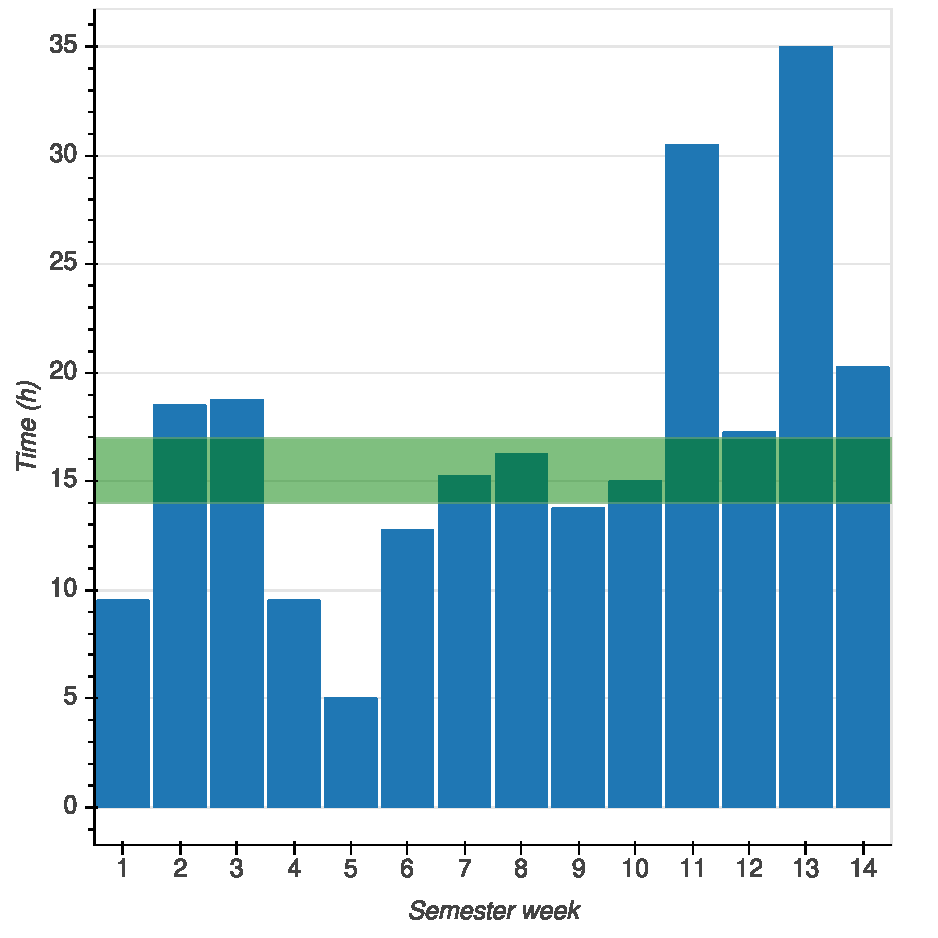
\includegraphics[width=\linewidth]{img/weekly.pdf}
  \end{figure}
\end{minipage}
\begin{minipage}[c]{0.2\linewidth}
  \begingroup
  \renewcommand{\arraystretch}{1}
  \begin{table}[H]
    \centering
    \begin{tabulary}{\linewidth}{rrl}
      \toprule
      Week & Time (h) & Comment\\
      \midrule
      1 & 10 & \\
      2 & 18 & \\
      3 & 19 & \\
      4 & 10 & \\
      5 & 5 & due to sickness \\
      6 & 13 & \\
      7 & 15 & \\
      8 & 16 & \\
      9 & 14 & \\
      10 & 15 & \\
      11 & 30 & \\
      12 & 17 & \\
      13 & 35 & \\
      14 & 20 & \\
      \midrule
      Total & 237 \\
      \bottomrule
    \end{tabulary}
  \end{table}
  \endgroup
\end{minipage}
\caption{Time spent per week}
\end{figure}

The time entries tracked were split into various categories:

\begin{table}[H]
  \begin{tabulary}{\linewidth}{lLr}
    \toprule
    Category & Description & Time (h) \\
    \midrule
    Documentation & Writing this documentation and working on API documentation. & 88 \\
    Implementation & Implementing the extension API, introducing mypy,
                     bugfixing. & 60 \\
    Contributions & Reviewing pull requests and contributions. & 34 \\
    Meetings & Meetings with Prof.~Stefan~Keller, language reviews with
               AnneMarie~O'Neill, video calls with Fritz~Reichwald (see section
               \ref{sec:team}). & 29 \\
    Other & Reading API design literature, communication with community, fixing
            issues with upstream library upgrades, etc. & 27 \\
    \bottomrule
  \end{tabulary}
  \caption{Time tracking categories}
\end{table}

Reviewing the time tracked per week per category, the project phases initially
defined in the schedule on page \pageref{img:schedule} are clearly apparent:

\vspace{1em}

\begin{figure}[H]
  \centering
  \makebox[\textwidth][c]{
    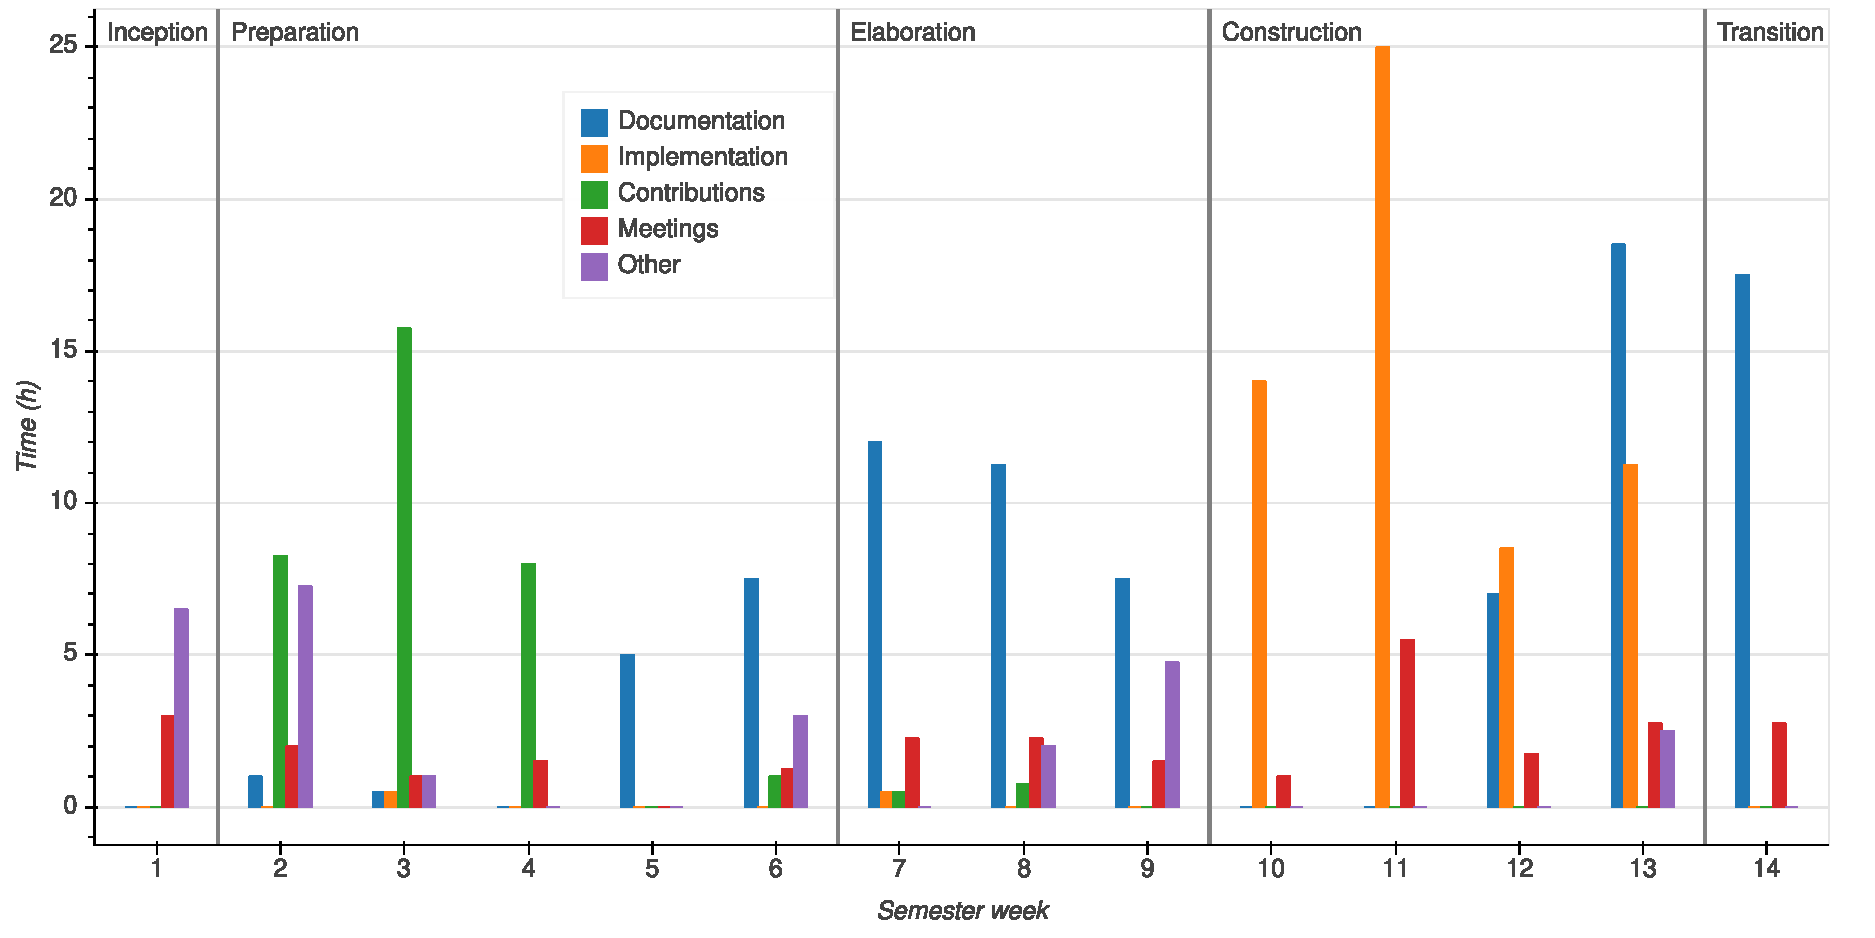
\includegraphics[width=1.2\linewidth]{img/topic.pdf}
  }
  % https://tex.stackexchange.com/a/16584/28697makebox[\textwidth][c]{
  \caption{Time tracking categories per week}
\end{figure}


% Codestatistik (Zeilen: Kommentare, Klassen, Packages)
\section{Code Statistics}
Since the work on this project was on an existing codebase, it is difficult to
distinguish in code statistics what work was pre-existing, compared to work done
as part of the project.

In the following table, code statistics as calculated by the
cloc\footnote{\url{https://github.com/AlDanial/cloc}} tool (``count lines of
code'') are presented for all files created as part of this project, as well as
files with major changes:

\begingroup
\renewcommand{\arraystretch}{1}
\begin{table}[H]
  \centering
  \begin{tabulary}{\linewidth}{rlrrrrr}
    \toprule
    Directory & File & Blank & Comment & Code & Func./Meth. & Classes \\
    \midrule
    api/ & \emph{Total} & 133 & 304 & 111 & 20 & 6 \\
    & \_\_init\_\_.py & 4 & 22 & 0 & 0 & 0 \\
    & apitypes.py & 3 & 19 & 5 & 0 & 0 \\
    & cmdutils.py & 59 & 108 & 52 & 6 & 3 \\
    & config.py & 8 & 29 & 6 & 1 & 0 \\
    & downloads.py & 20 & 33 & 22 & 3 & 1 \\
    & hook.py & 26 & 46 & 20 & 8 & 2 \\
    & interceptor.py & 10 & 28 & 5 & 2 & 0 \\
    & message.py & 3 & 19 & 1 & 0 & 0\vspace{1em} \\
    components/ & \emph{Total} & 213 & 338 & 556 & 65 & 2 \\
    & \_\_init\_\_.py & 2 & 18 & 0 & 0 & 0 \\
    & adblock.py & 64 & 76 & 207 & 19 & 2 \\
    & caretcommands.py & 52 & 72 & 87 & 18 & 0 \\
    & misccommands.py & 61 & 91 & 160 & 21 & 0 \\
    & scrollcommands.py & 20 & 44 & 58 & 4 & 0 \\
    & zoomcommands.py & 14 & 37 & 44 & 3 & 0\vspace{1em} \\
    extensions/ & \emph{Total} & 70 & 68 & 112 & 13 & 4 \\
    & interceptors.py & 20 & 24 & 19 & 3 & 1 \\
    & loader.py & 50 & 44 & 93 & 10 & 3\vspace{1em} \\
    browser/ & browsertab.py & 256 & 251 & 617 & 136 & 15 \\
    commands/ & command.py & 75 & 130 & 371 & 20 & 2 \\
    \bottomrule
  \end{tabulary}
  \caption{Line count for added/changed modules}
  \label{tab:coverage}
\end{table}
\endgroup

Notes:

\begin{itemize}[parsep=5pt]

  \item \verb|browser/browsertab.py| is relatively large for a single file.
    Should any additions be required in the future, it should be split into smaller
    files.
  \item \verb|__init__.py| files mark a folder as a Python package, thus
    do not contain any code.
  \item Some files in \verb|api/| only import code from internal
    qutebrowser modules in order to expose them to the extension API, and thus
    do not contain any functions/classes on their own.
  \item Documentation (such as the API documentation in appendix \ref{ch:sphinx}
    or the user documentation for qutebrowser commands) is generated from
    Python docstrings in the code, which cloc counts as ``comments''.
\end{itemize}

\section{Demo extension}
In this section, a demo extension using various aspects of the API is
presented. The extension checks whether a website uses the
Leaflet\footnote{\url{https://leafletjs.com/}} JavaScript library, which is
often used to embed OpenStreetMap\footnote{\url{https://www.openstreetmap.org/}}
maps into websites.

First, the extension imports the \verb|typing| module from Python's standard
library, and various submodules of the \verb|qutebrowser.api| module:

\begin{minted}[linenos]{python}
import typing

from qutebrowser.api import cmdutils, apitypes, hook, message
\end{minted}

Next, it registers a command handler using the \py{@cmdutils.register()}
decorator, which causes the function to be available to the user as a
\verb|:has-leaflet| command inside qutebrowser:

\begin{minted}[linenos,firstnumber=6]{python}
@cmdutils.register()
@cmdutils.argument('tab', value=cmdutils.Value.cur_tab)
def has_leaflet(tab: apitypes.Tab) -> None:
    """Check whether a website uses leaflet."""
\end{minted}

The command name is automatically deduced from the name of the function, while
the Python docstring also gets shown in qutebrowser's command completion:

\begin{figure}[H]
  \centering
  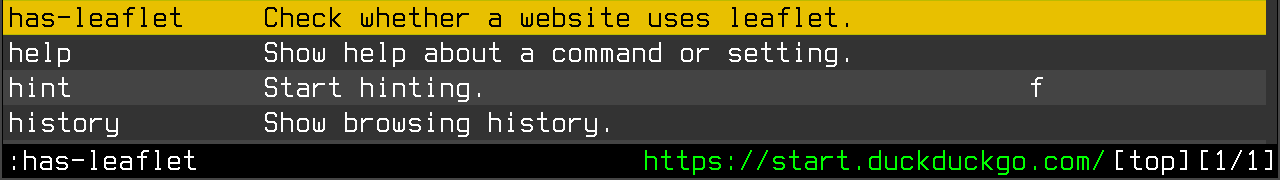
\includegraphics[width=\linewidth]{img/screenshot-completion.png}
  \caption{Command completion showing the \texttt{:has-leaflet} command.}
\end{figure}

The \py{@cmdutils.argument(...)} decorator is used to pass more information
about the \verb|tab| argument to the API. Due to the
\py{value=cmdutils.Value.cur_tab} parameter, the \verb|tab| argument is set to
the tab object of the tab currently being focused when qutebrowser calls the
command handler.

Next, the extension uses the tab API to find HTML elements on the website:

\begin{minted}[linenos,firstnumber=10]{python}
    tab.elements.find_css('.leaflet-container',
                          callback=show_message,
                          error_cb=show_error_message)
\end{minted}

The \verb|find_css()| method takes three arguments: A CSS selector, a callback
which gets called on success, and a callback which gets called in case of an
error.

The CSS class selector \verb|.leaflet-container| is used to find websites using
Leaflet, as the library uses that selector for its map display.

The callback used for errors simply uses the \verb|message| module to show an
error message to the user:

\begin{minted}[linenos,firstnumber=15]{python}
def show_error_message(error: str) -> None:
    message.error(str(error))
\end{minted}

The callback called on success instead checks whether the \verb|elements| lists
it received contains any elements. Depending on the result, it shows the
appropriate message:

\begin{minted}[linenos,firstnumber=19]{python}
def show_message(elements: typing.List[apitypes.WebElement]) -> None:
    if elements:
        message.info("Yay, this site uses Leaflet!")
    else:
        message.info("This site does not use Leaflet...")
\end{minted}

Finally, the extension uses the \py{@hook.init()} decorator to define an
initialization hook. There, it displays an ``osmtest initialized'' message:

\begin{minted}[linenos,firstnumber=26]{python}
@hook.init()
def init(_context: apitypes.InitContext) -> None:
    message.info("osmtest initialized")
\end{minted}

Note that it receives an \verb|InitContext| object with additional information
(such as commandline arguments). Since the argument is unused, its name is
prefixed by an underscore, a common convention in Python code.

The full code of the demo extension can be found on page \pageref{lst:demo}.\\[2em]

\begin{figure}[H]
  \centering
  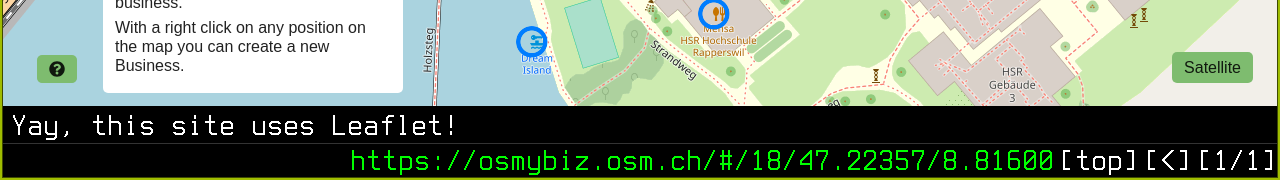
\includegraphics[width=\linewidth]{img/screenshot-leaflet.png}
  \caption{Running the \texttt{:has-leaflet} command on OSMyBiz.}
\end{figure}

\begin{figure}[H]
  \centering
  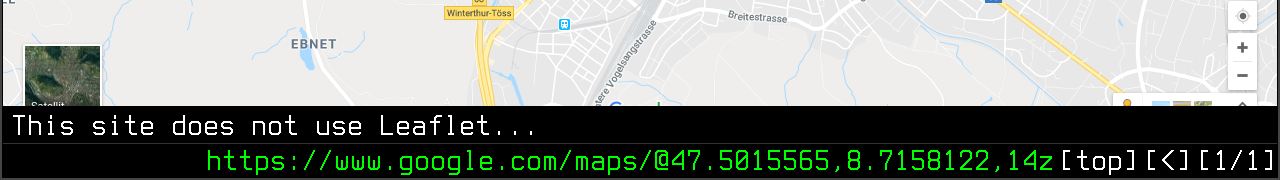
\includegraphics[width=\linewidth]{img/screenshot-leaflet-no.png}
  \caption{Running the \texttt{:has-leaflet} command on Google Maps.}
\end{figure}


\begin{listing}[b]
\centering
\begin{minted}[linenos]{python}
import typing

from qutebrowser.api import cmdutils, apitypes, hook, message


@cmdutils.register()
@cmdutils.argument('tab', value=cmdutils.Value.cur_tab)
def has_leaflet(tab: apitypes.Tab) -> None:
    """Check whether a website uses leaflet."""
    tab.elements.find_css('.leaflet-container',
                          callback=show_message,
                          error_cb=show_error_message)


def show_error_message(error: str) -> None:
    message.error(str(error))


def show_message(elements: typing.List[apitypes.WebElement]) -> None:
    if elements:
        message.info("Yay, this site uses Leaflet!")
    else:
        message.info("This site does not use Leaflet...")


@hook.init()
def init(_context: apitypes.InitContext) -> None:
    message.info("osmtest initialized")
\end{minted}
\caption{Demo extension}
\label{lst:demo}
\end{listing}

% Ausblick: Weiterentwicklung (nur wichtigste Punkte)
\section{Future Work}
While there was a lot of progress for extensions in qutebrowser, there is plenty
of room for future research and improvements:

\begin{itemize}
  \item The core of qutebrowser should be further modularized. Ideally, its
    architecture would be designed with the microkernel pattern \autocite[171ff]{posa1}
    for operating systems in mind, however, the resulting extension API should
    always be general enough to be useful for more than one use-case.
  \item After the extension API is stable enough, extensions should be made open
    for third-party contributions, initially by allowing users to download
    extensions they want to use in a folder such as
    \verb|~/.local/share/qutebrowser/extensions|.
  \item Many use-cases and ideas for extensions have been
    suggested\footnote{\url{https://github.com/qutebrowser/qutebrowser/issues/30}}
    by qutebrowser's users. These should be carefully reviewed and considered
    for future API additions.
  \item In order to foster community involvement around extensions and keep
    users safe, a central place to distribute and update extensions should
    exist. Furthermore, an ``extension store'' should be added to qutebrowser,
    which allows users to easily discover, install and upgrade extensions.
\end{itemize}

The currently existing API has been designed with future additions in mind: The
\verb|downloads.py| module currently only allows triggering a temporary
download, but was split off from other modules in order to allow for future
additions for handling user-initiated downloads. Furthermore, init-hooks which
can be defined by extensions receive a special \verb|InitContext| instance
(rather than getting called with the information therein as individual
arguments) so that the \verb|InitContext| class can be extended in the future
without extensions needing to adjust their code.

% From project management part:
% % Resultate und Weiterentwicklung
% \chapter{Results and Future Work}
% 
% % Resultate (ev. nach oben in Teil I Kap. 5 eingleidern)
% \section{Results}
% 
% % Möglichkeiten der Weiterentwicklung
% \section{Possible Future Work}
% 
% % Vorgehen (welche Mögl. würde man nun wie weiterentwickeln?)
% \section{Future Approach}



% Persönliche Berichte
\section{Personal Review}
Exactly one week before this project was due, December \nth{14} 2018,
qutebrowser celebrated its fifth birthday. Back then, I was not sure whether I
wanted to pursue a Bachelor's degree at all, or whether I would rather work in
the industry immediately. Later, when it was clear that I wanted to study at
HSR, I wondered whether I would ever have the chance to work on qutebrowser as
part of my studies.

I was happy that this was indeed the case, thanks to the flexibility of the
HSR and Prof.~Stefan~Keller. There are a lot of other interesting research
project proposals, so I am honored that this arrangement was possible.

Working on an existing project proved to be challenging, as it was a ``moving
target'' at times with many external contributors involved. Even though I
planned a phase at the beginning for reviewing existing contributions, it became
apparent that reviews would take much longer. Additionally, contributions
continued despite a notice asking people to hold them back if possible. In
retrospective, a better idea would be to put up such a notice very early,
shorten the time for reviews of existing contributions, and deal with the merge
conflicts after the research project finished as appropriate.

I decided to write this report in English so it is widely accessible by
qutebrowser users and developers -- I hope some of them will find the time to
read it, and enjoy reading it as much as I enjoyed writing it. I initially was
hesitant because I never wrote something of this scale in a foreign language
before, but I quickly discovered that I was equally comfortable with writing
English and writing German (my native language).

All in all, I am pleased with how things turned out, even if this is only the
first step of many needed for proper extension support in qutebrowser. I hope I
will soon be able to continue working towards this goal.

% Dank
\section{Acknowledgements}
Working on an open-source project with an idea contributed by a student, as well
as doing an SA as a single person, is rather untypical. I am very grateful that
Prof.~Stefan~Keller was open to mentor this project as an advisor despite the
unusual conditions. His support and insights in our regular meetings were
invaluable.

Thanks to the qutebrowser community for making qutebrowser into far more than
just a personal pet project of mine. Without this community, I doubt I would
still be working on it after five years -- when I started, I never imagined that
it would get that far.

I am thankful to all qutebrowser contributors for their patience and
understanding when I could not attend to their contributions in a timely manner
while working on this project.

I would especially like to thank Fritz~Reichwald for his contributions towards
switching to the Sphinx documentation generator, even though I did not end up
using his work in the scope of this project. We plan to meet up and merge the
two approaches soon, so the entire qutebrowser documentation can be converted to
Sphinx.

Thanks to AnneMarie~O'Neill for her careful English reviews and constructive
feedback on possible improvements. Her suggestions were always very welcome and
accurate.

Last but not least, thanks to Méline~Sieber for her constant encouragement
throughout the semester, and for always helping me out of the maze when I got
stuck somewhere. You were here when I needed it, \emph{``für jede Meile bis zur
letzten''}.


